\chapter{Demonstration Problem: Hypersonic Retro-firing Annular Jet}
\label{chapter-five}

To demonstrate the advantages and the robustness of the decoupled flow and
adjoint solvers relative to the fully coupled flow and adjoint solvers, a
demonstration problem is chosen with sufficiently challenging physics.  The
problem must include a sufficient sensitivity to the chemistry model to
highlight the stability concerns of the decoupled flow solver presented in
\sref{sec:15-kps-sphere-cone}.  In this case, the sensitivity manifests through
the formation of a large, recirculating buffer gas zone that covers most of the
vehicle outer surface. This chapter details the geometry and test conditions of
the demonstration problem, as well as the characteristics of the flow solution.

\section{Annular Jet Configuration and Test Conditions}

The geometry chosen is a hypersonic re-entry vehicle with a retro-firing annular
nozzle, as shown in \fref{fig:annular-jet-side}.
%------------------------------------------------------------------------------%
\begin{figure}[h]
  \centering
	\begin{subfigure}[b]{0.4\textwidth}
    \centering
    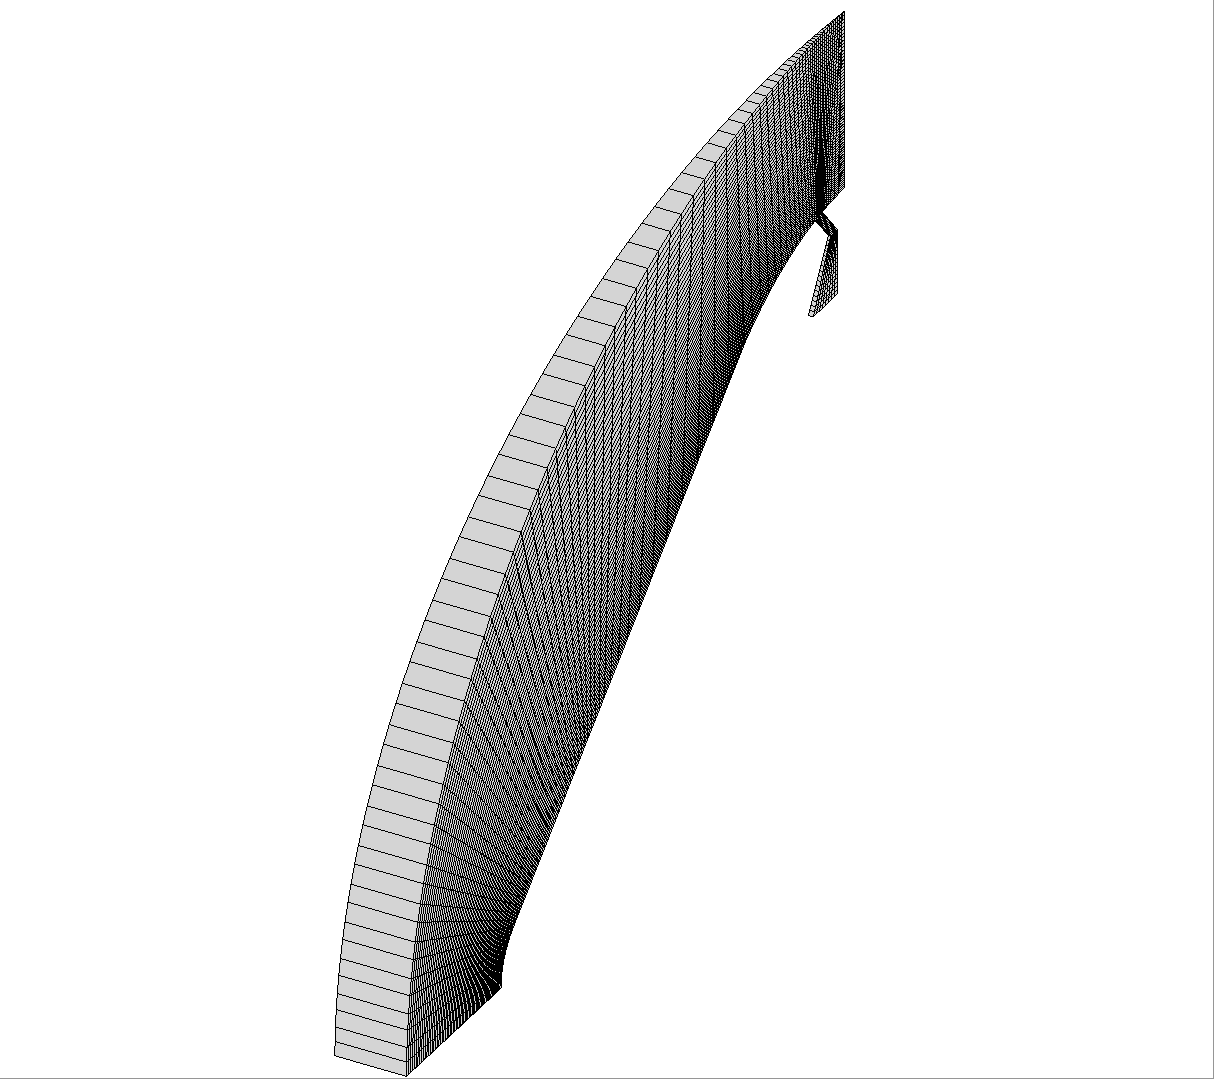
\includegraphics[width=\textwidth]{figures/iso-coarse.png}
  \end{subfigure}
	\begin{subfigure}[b]{0.4\textwidth}
    \centering
    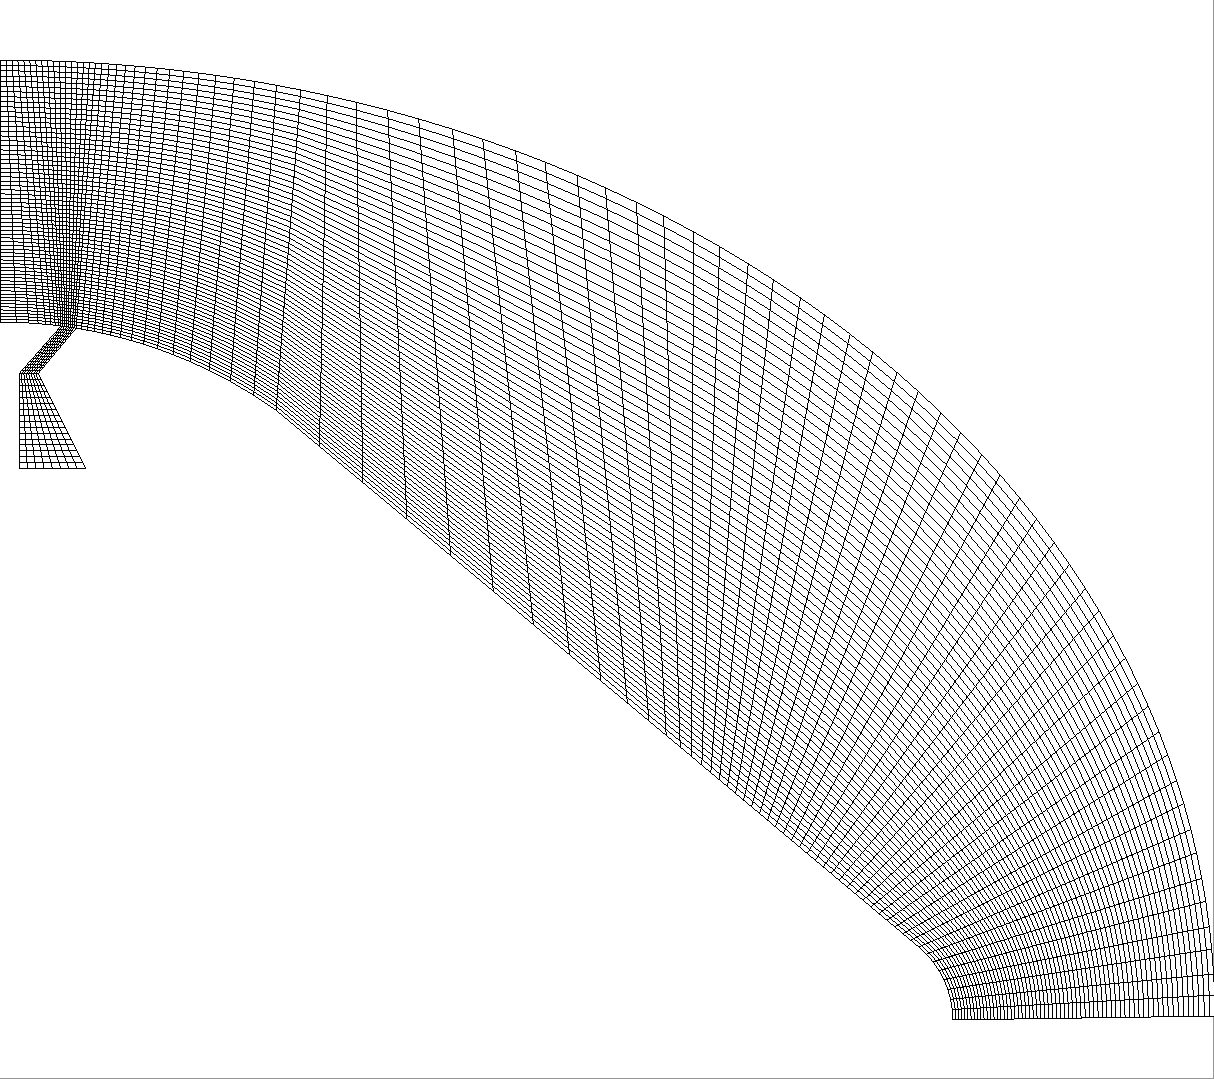
\includegraphics[width=\textwidth]{figures/side-coarse.png}
  \end{subfigure}
  \caption{Annular jet geometry.}
  \label{fig:annular-jet-side}
\end{figure}
%------------------------------------------------------------------------------%
This geometry has been investigated by Gnoffo et al.\cite{gnoffo2016tapping} to
increase drag from ``pulsing'' the annular jet to obtain a beneficial effect
from the unsteady shock interaction with the plume of the jet.  In the
aforementioned work, it has been determined that a steady solution to the Euler
equations exists for this annular jet configuration.  This problem is attractive
for optimization, because the annular jet plenum conditions significantly affect
aerodynamic and aerothermodynamic quantities of interest on the vehicle surface.
These effects are very non-linear, due to the shock and jet plume interaction,
and it is therefore very difficult to intuitively understand the relationship
between the plenum conditions and vehicle surface quantities.  Because the
adjoint solver is rigorously derived from the discretized governing equations,
the relationship between the plenum and surface can be directly determined,
making this an excellent showcase problem for adjoint-based sensitivity
information.

%------------------------------------------------------------------------------%
\begin{table}[h]
  \centering
  \begin{tabular}{c|c|c}
    Parameter & Description & Value \\
    \hline
    $r_{throat}$       &   nozzle throat radius, $m$                 & 0.02 \\
    $r_{plenum,inner}$ &   inside nozzle radius at plenum face, $m$  & 0.02 \\
    $r_{plenum,outer}$ &   outside nozzle radius at plenum face, $m$ & 0.07 \\
    $r_{exit,inner}$   &   inside nozzle radius at exit, $m$         & 0.064 \\
    $r_{exit,outer}$   &   outside nozzle radius at exit, $m$        & 0.08 \\
    $l_{conv}$         &   distance from plenum to throat, $m$       & 0.05 \\
    $\theta_c$         &   cone half angle, deg                      & 50.0
  \end{tabular}
  \caption{Annular nozzle geometry inputs.}
  \label{tab:annular-geom}
\end{table}
%------------------------------------------------------------------------------%
The geometry is described by the parameters shown in \tref{tab:annular-geom},
with the mesh originally created as a structured grid and then converted to an
unstructured grid comprised of hexahedra and prismatic elements.  The flow
conditions corresponding to a Mach 20 freestream flow are shown in
\tref{tab:flow-conditions}, with all simulations conducted using a 9-species
Hydrogen-air mixture comprised of $H_2$, $N_2$, $O_2$, $H$, $N$, $O$, $NO$,
$OH$, and $H_2 O$.
%------------------------------------------------------------------------------%
\begin{table}[!h]
  \centering
  \begin{tabular}{c|c|c}
    Flow Condition & Description & Value \\
    \hline
    $V_{\infty}$    & freestream velocity, $m/s$        & 5686.24 \\
    $\rho_{\infty}$ & freestream density, $kg/m^3$      & 0.001 \\
    $T_{\infty}$    & freestream temperature, $K$       & 200.0 \\
    $M_{\infty}$    & freestream Mach number (derived)  & 20.0
  \end{tabular}
  \caption{Flow conditions.}
  \label{tab:flow-conditions}
\end{table}
%------------------------------------------------------------------------------%

\section{Annular Jet Flow Features and Steadiness Dependence on Cone Angle}

\frefs{fig:cone-angle-temperature}{fig:cone-angle-water} show contours for
annular plenum blowing pure hydrogen at 200,000 $Pa$ and 500$K$, and illustrate the
complexity of the physics associated with this annular jet configuration.  The
temperature contours in \fref{fig:cone-angle-temperature} show that the annular
jet configuration creates a buffer gas region behind the bow shock.  This buffer
gas provides a beneficial cooling mechanism for the outer surface of the
vehicle.  The production of water can be seen in \fref{fig:cone-angle-water},
with the overlayed streamlines indicating that a separation bubble forms just
downstream of the annular nozzle exit.  The degree of separation in this flow is
sensitive to the cone angle of the vehicle, and it has been observed that
lowering the cone angle reduces the size of this separation bubble.
%------------------------------------------------------------------------------%
\begin{figure}[h!]
  \centering
  \begin{subfigure}{0.45\textwidth}
    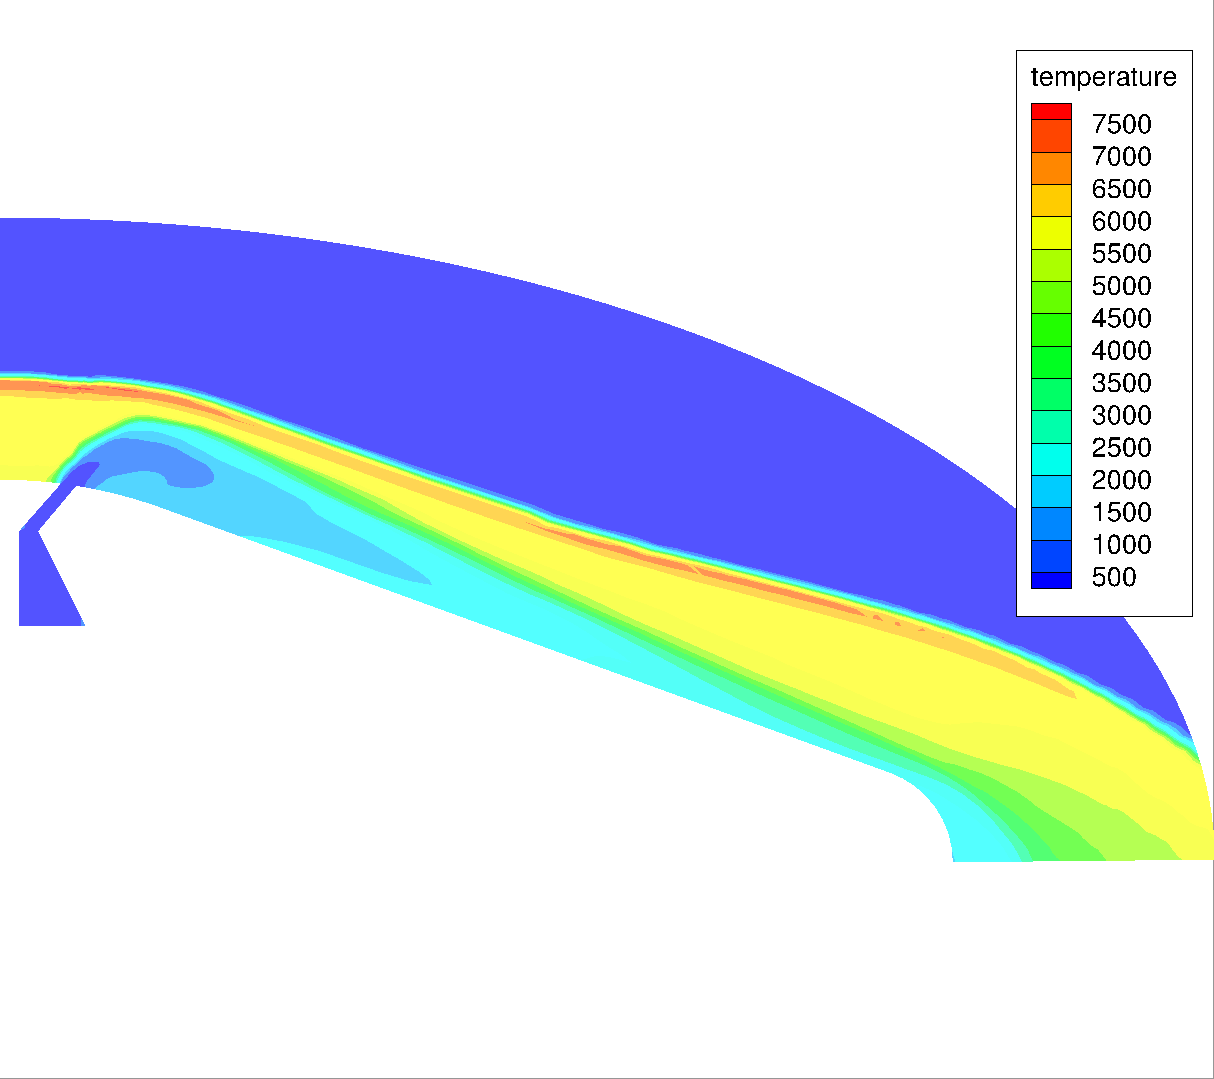
\includegraphics[width=\textwidth]{figures/srp/70deg-temperature.png}
    \caption{$70^o$ Cone angle}
    \label{fig:70deg-temperature-contour}
  \end{subfigure}
  \begin{subfigure}{0.45\textwidth}
    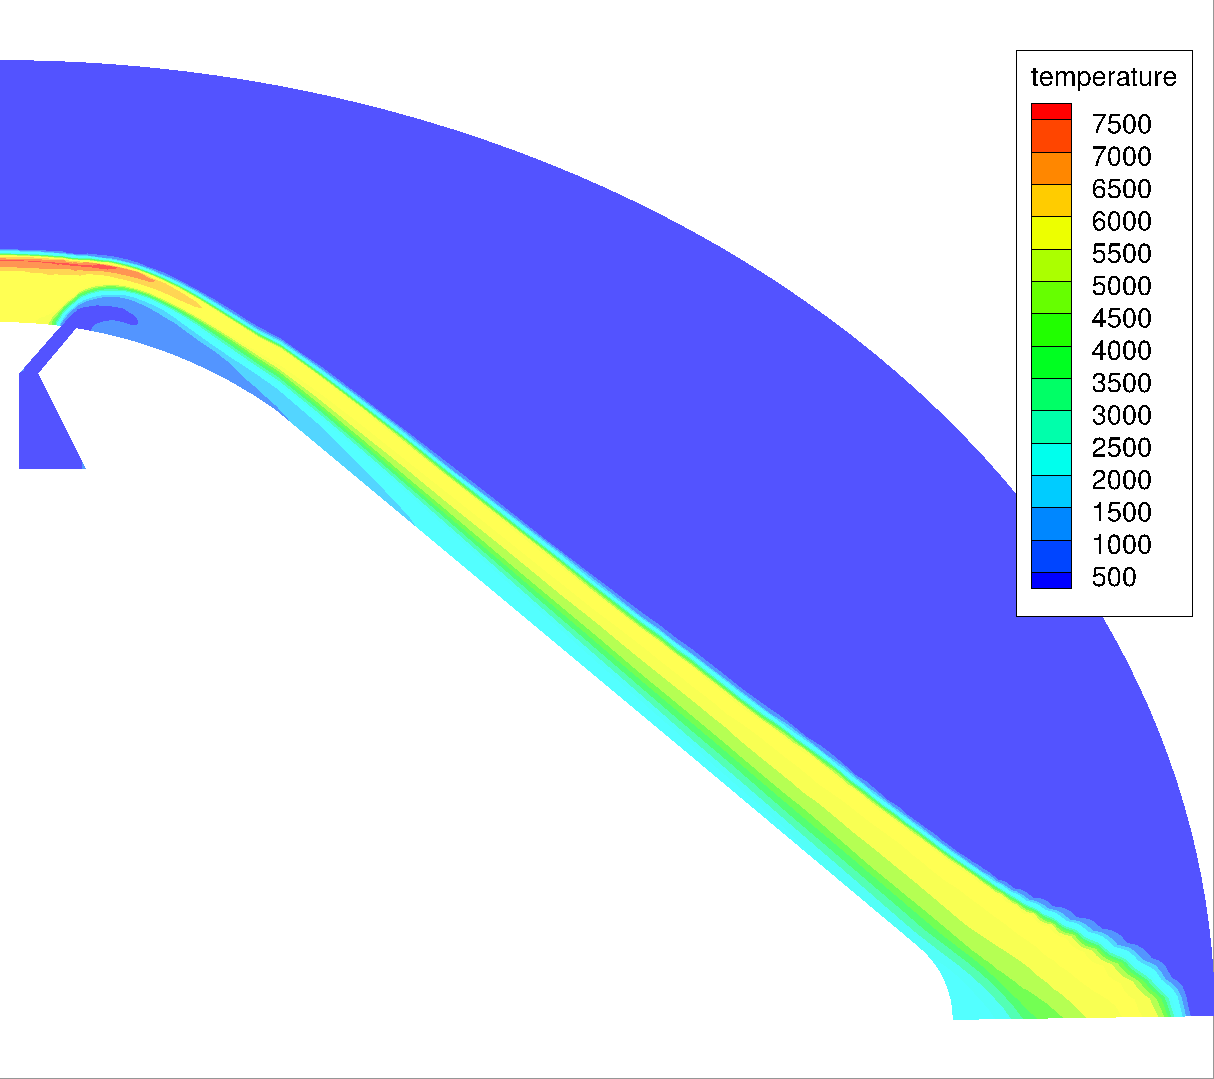
\includegraphics[width=\textwidth]{figures/srp/50deg-temperature.png}
    \caption{$50^o$ Cone angle}
    \label{fig:50deg-temperature-contour}
  \end{subfigure}
  \caption{Annular jet temperature contours, blowing pure $H_2$.}
  \label{fig:cone-angle-temperature}
\end{figure}
%------------------------------------------------------------------------------%
%------------------------------------------------------------------------------%
\begin{figure}[h!]
  \centering
  \begin{subfigure}{0.45\textwidth}
    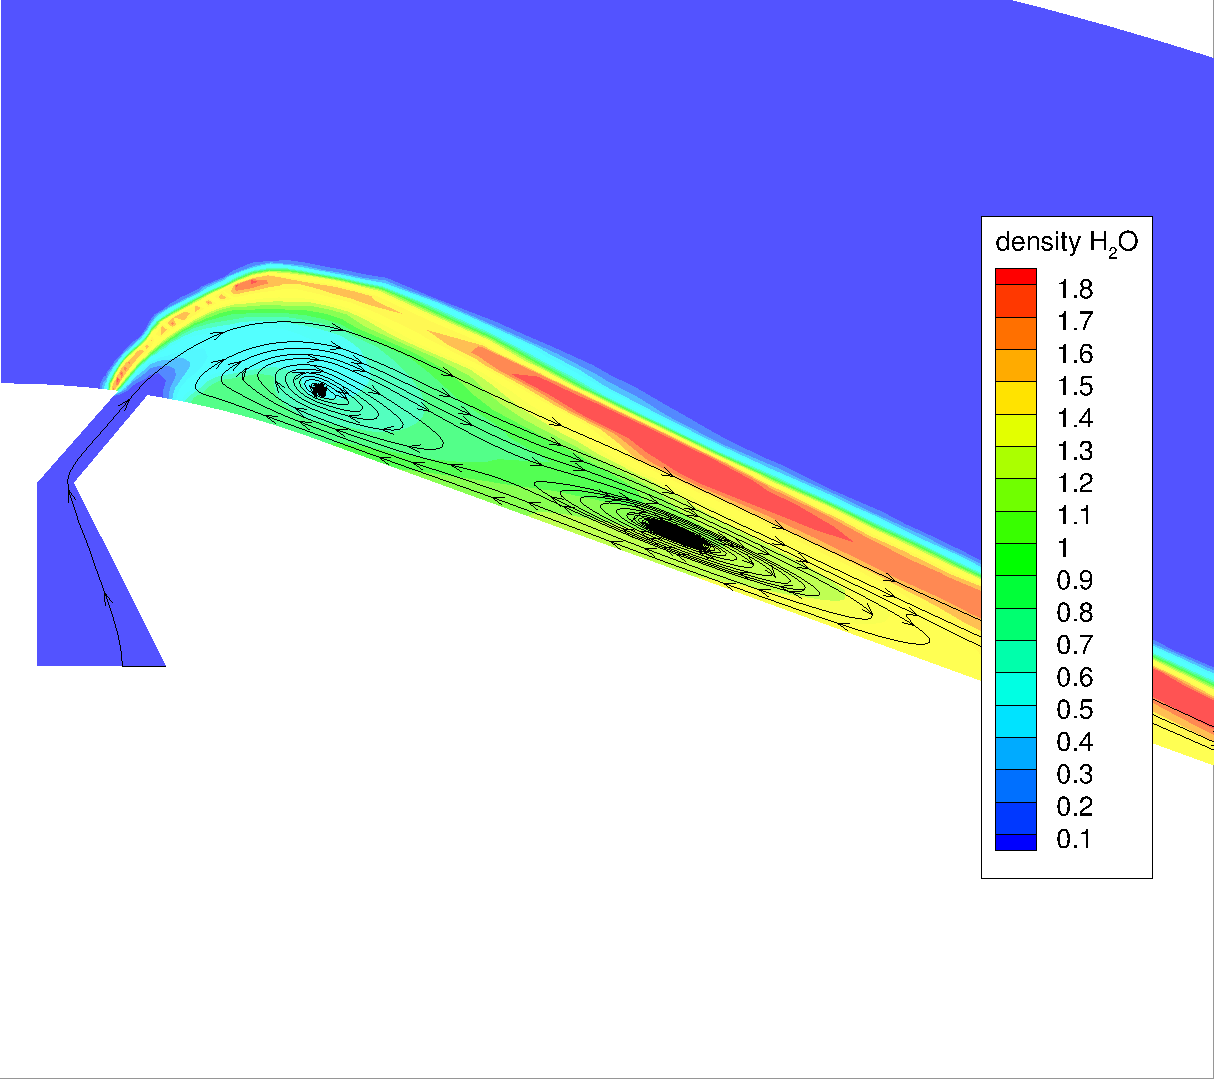
\includegraphics[width=\textwidth]{figures/srp/70deg-water.png}
    \caption{$70^o$ Cone angle}
    \label{fig:70deg-water-contour}
  \end{subfigure}
  \begin{subfigure}{0.45\textwidth}
    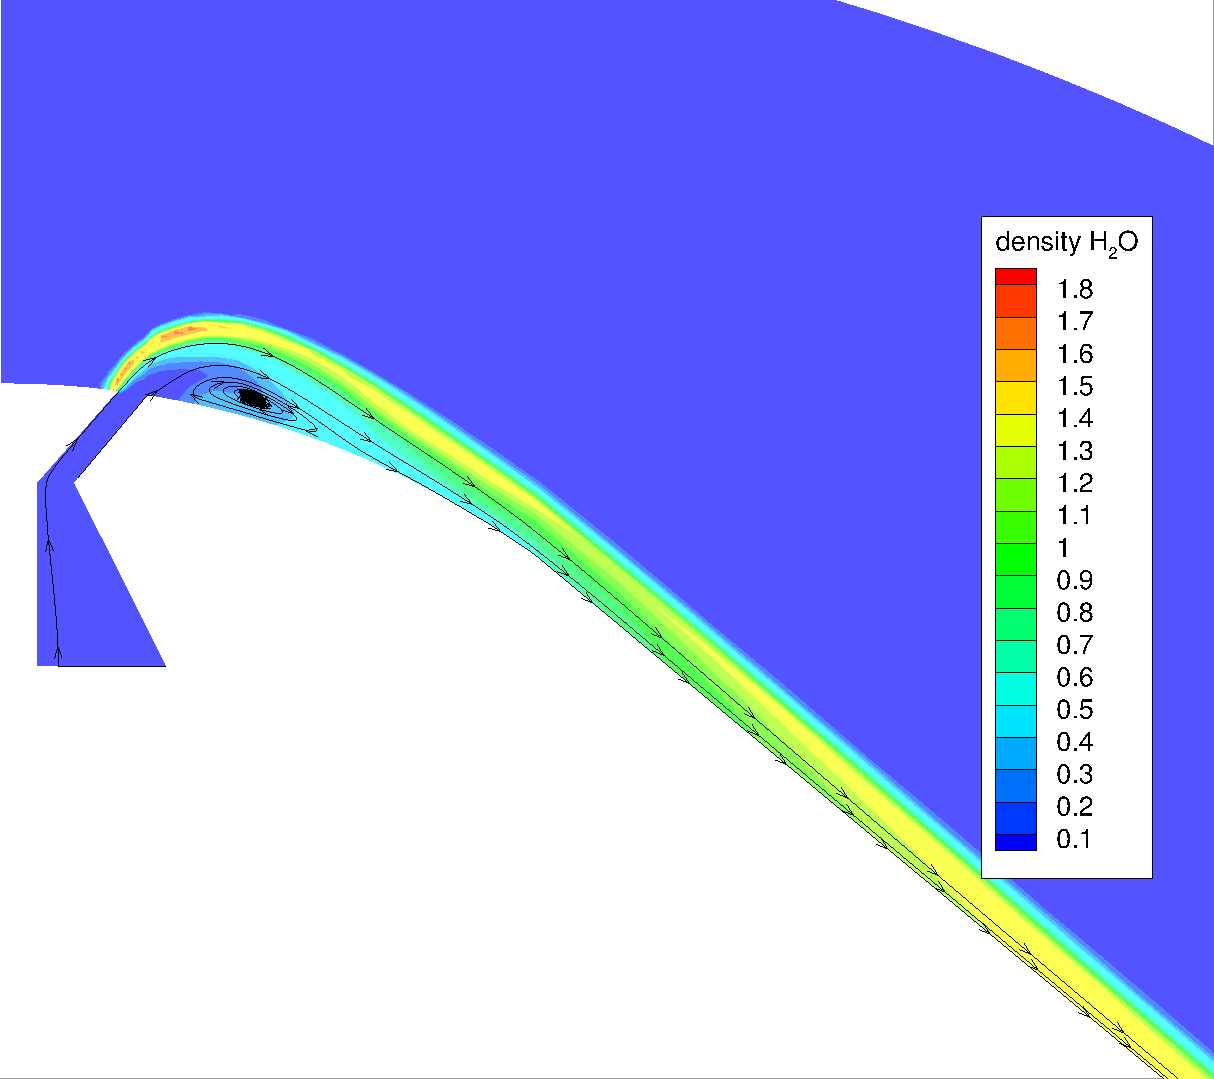
\includegraphics[width=\textwidth]{figures/srp/50deg-water.png}
    \caption{$50^o$ Cone angle}
    \label{fig:50deg-water-contour}
  \end{subfigure}
  \caption{Annular jet $H_2 O$ density contours, blowing pure $H_2$.}
  \label{fig:cone-angle-water}
\end{figure}
%------------------------------------------------------------------------------%

The size of the separation bubble shown in \fref{fig:cone-angle-water} has
implications on the steadiness of the flow.  While the reacting gas path of the
FUN3D flow solver has the capability to simulate unsteady flows, the newly
developed FUN3D reacting gas adjoint solver is currently limited in scope to
steady flows.  A full design optimization covers a wide variety of flow
solutions, and it is therefore important to verify that the geometry chosen
results in steady flow for all design perturbations.  A $70^o$ cone angle was
initially chosen, instead of $50^o$, because of a rich history of investigation
associated with the Mars Pathfinder probe\cite{gnoffo1996influence}.  It was
heuristically determined that blowing a light gas with a high cone angle leads
to a sonic corner body, a state where the sonic line extends the shoulder of the
vehicle.  Numerical experiments indicate that the annular jet is susceptible to
very low frequency and low amplitude pulsing of the entrained separation bubble
on sonic corner bodies, where the separation bubble near the nozzle exit is
relatively large.
%------------------------------------------------------------------------------%
\begin{figure}[h]
  \centering
  \begin{subfigure}[b]{0.45\textwidth}
    \centering
    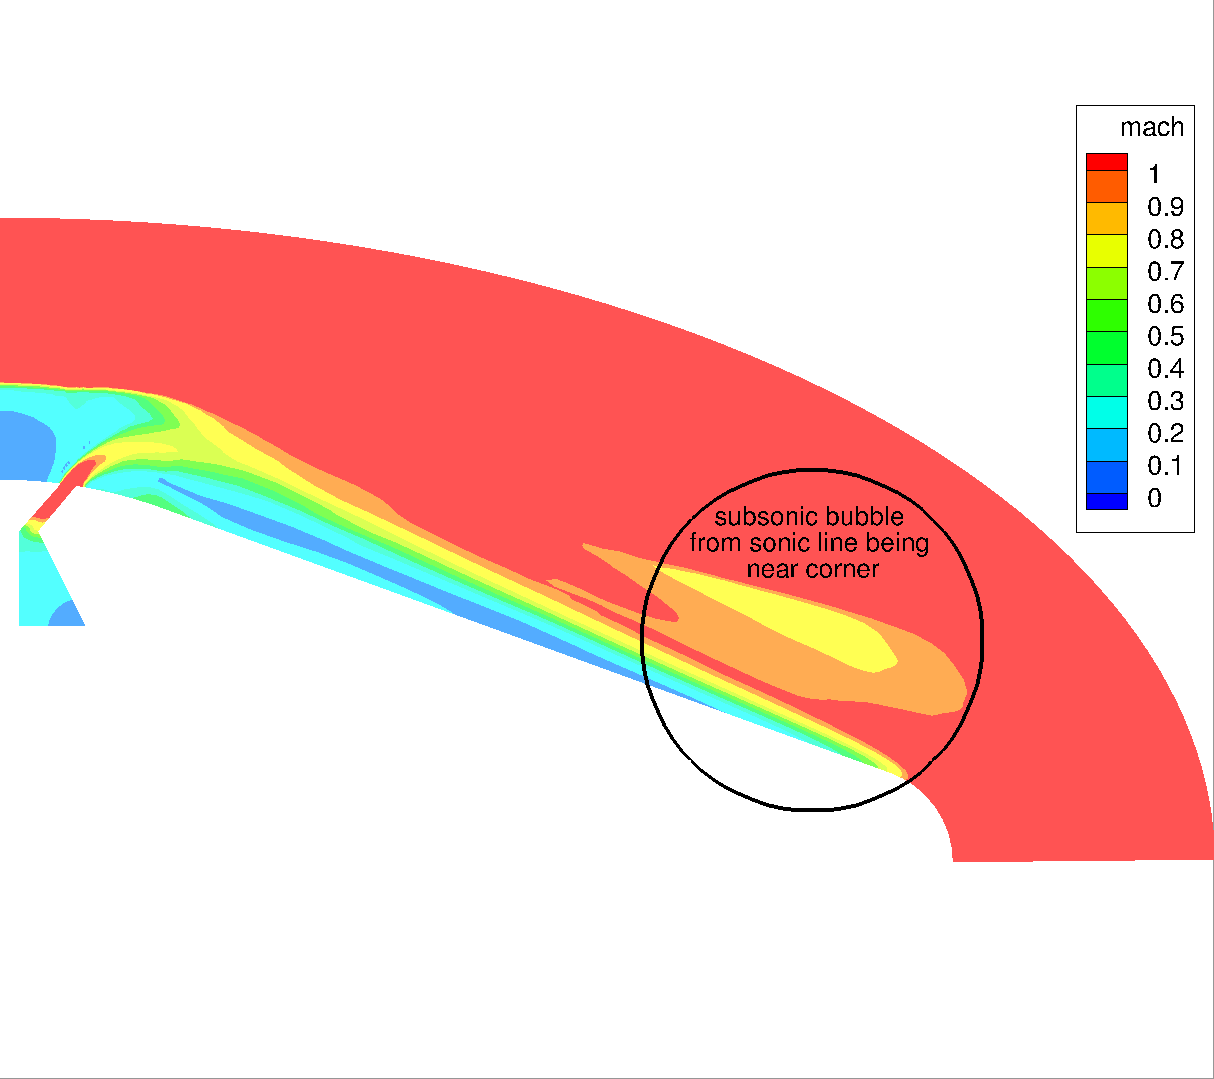
\includegraphics[width=\textwidth]{figures/sonic-bubble/sonic_bubble.png}
    \caption{$70^o$ Cone angle}
    \label{fig:70-deg-cone}
  \end{subfigure}
  \begin{subfigure}[b]{0.45\textwidth}
    \centering
    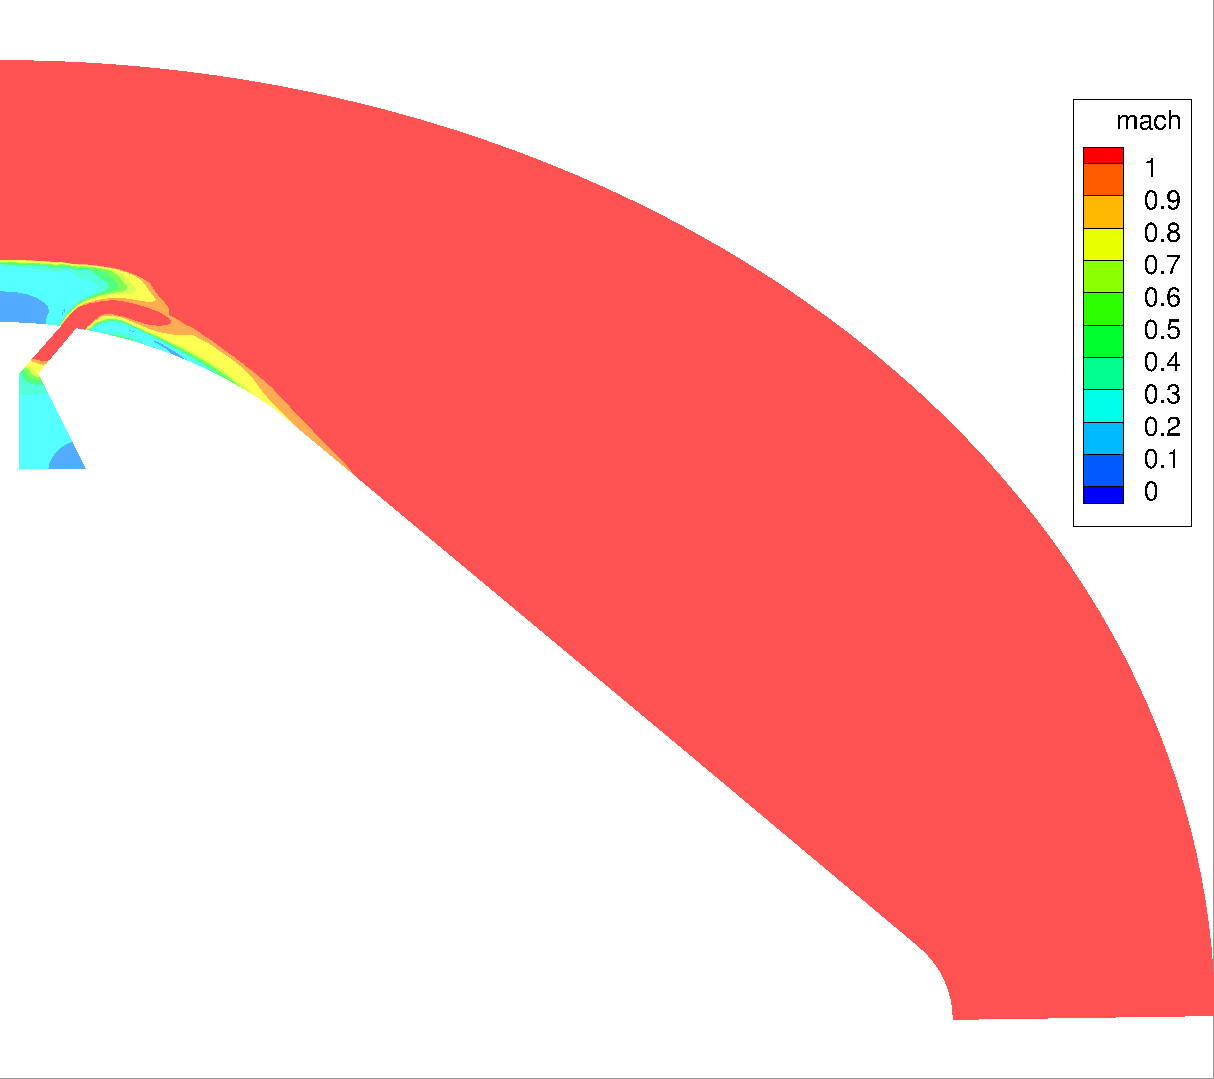
\includegraphics[width=\textwidth]{figures/sonic-bubble/no_bubble.png}
    \caption{$50^o$ Cone angle}
    \label{fig:50-deg-cone}
  \end{subfigure}
  \caption{Annular jet sonic line comparison, blowing pure $H_2$.}
  \label{fig:cone-angle-comp}
\end{figure}
%------------------------------------------------------------------------------%
\fref{fig:cone-angle-comp} shows a comparison of mach number for the same flow
conditions as those in \frefs{fig:cone-angle-temperature}{fig:cone-angle-water}.
\fref{fig:70-deg-cone} highlights the subsonic bubble that is indicative of a
sonic corner body, whereas \fref{fig:50-deg-cone} shows that decreasing the cone
angle moves the sonic line upstream and eliminates the subsonic bubble.  The
strong dependence between the position of the sonic line on the vehicle and the
cone angle is the primary reason that the cone angle was chosen to be decreased
to $50^o$, rather that using the $70^o$ chosen by Gnoffo et
al.\cite{gnoffo2016tapping}.  The comparison between the $50^o$ and $70^o$ cone
angle geometries was done for a wide range of plenum conditions spanning the
design space to be discussed in the next chapter, and no subsonic bubble was
ever found for the $50^o$ cone angle.

\section{Mesh Refinement Study}
\label{sec:mesh-refinement-study}

To determine the sensitivity of the flow solution to mesh density, a grid
convergence study was attempted by uniformly refining the original mesh, using
the cut-cell method developed by Park\cite{park2008anisotropic} that uniformly
subdivides each element in the mesh.
%------------------------------------------------------------------------------%
\begin{table}[h]
  \centering
  \begin{tabular}{c|c}
    Plenum Condition & Value \\
    \hline
    Plenum Pressure, $P_{p,o}$, Pa   & 200,000 \\
    Plenum Temperature, $T_{p,o}$, K &  500 \\
    Plenum Fuel-Air Ratio $\fa$      &  0.7
  \end{tabular}
  \caption{Plenum conditions.}
  \label{tab:plenum-conditions}
\end{table}
%------------------------------------------------------------------------------%
The solution on each grid level was computed using the freestream conditions in
\tref{tab:flow-conditions} and the plenum conditions in
\tref{tab:plenum-conditions}. \fref{fig:mesh-refined} shows the progression
of refined meshes generated by this method,
%------------------------------------------------------------------------------%
\begin{figure}[h]
  \centering
  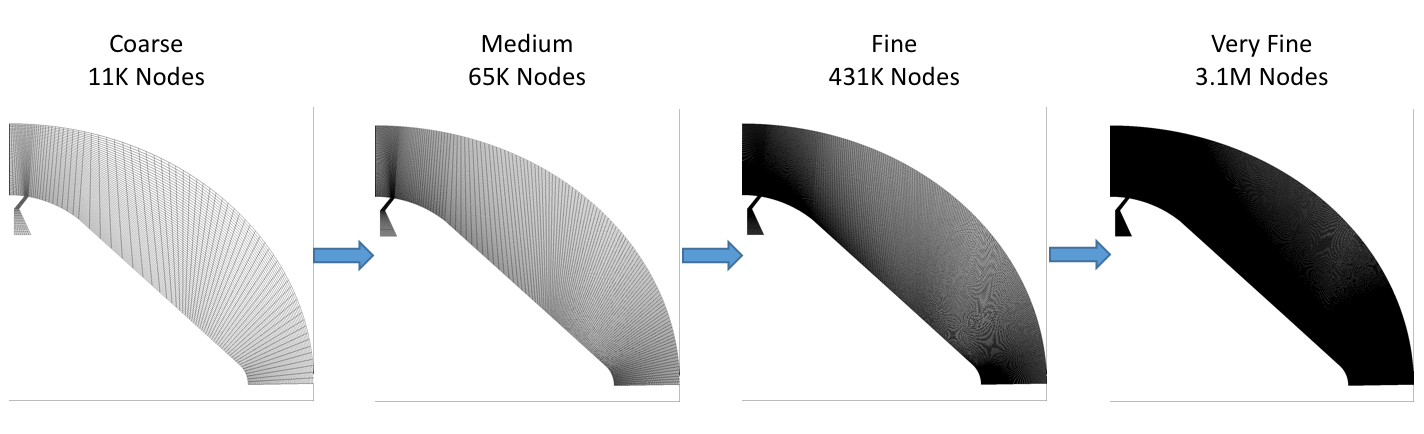
\includegraphics[width=\textwidth]{figures/mesh-progression.png}
  \caption{Uniformly refined meshes.}
  \label{fig:mesh-refined}
\end{figure}
%------------------------------------------------------------------------------%
and \fref{fig:grid-convergence} shows the grid convergence of surface
temperature and plenum mass flow rate for a nominal case.
%------------------------------------------------------------------------------%
\begin{figure}[!h]
  \centering
  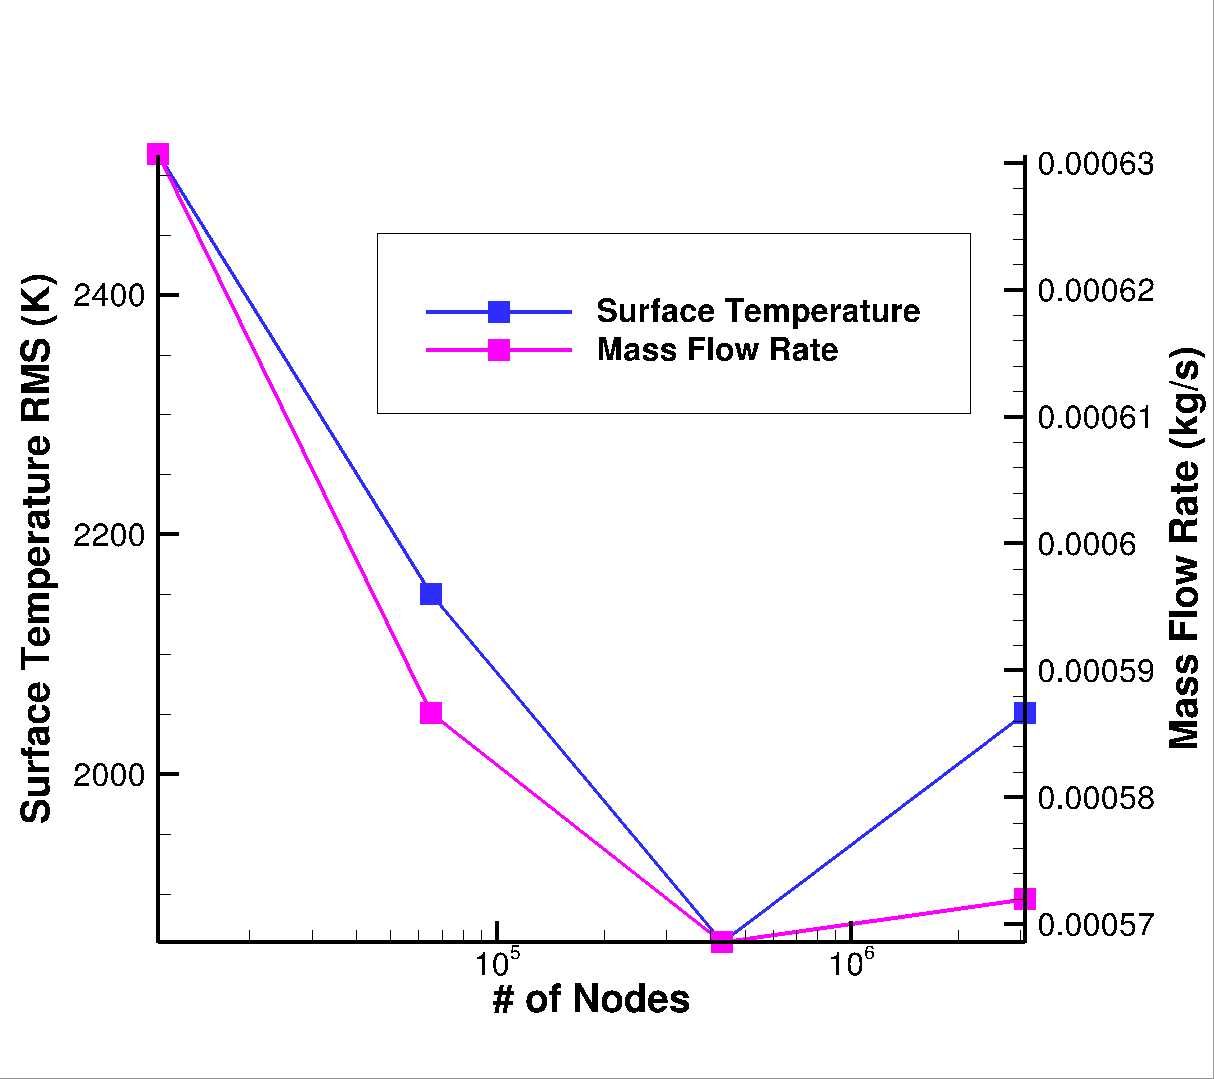
\includegraphics[width=0.5\textwidth]{figures/t-m-conv.png}
  \caption{Grid convergence.}
  \label{fig:grid-convergence}
\end{figure}
%------------------------------------------------------------------------------%
On the fine mesh ($431,000$ nodes), a frozen limiter was required to maintain
steady flow.  The flow solution for the very fine mesh ($3,100,000$ nodes) was
very unsteady, and freezing the flux limiter did not recover a steady flow
solution.  The values for surface temperature and mass flow rate on the very
fine mesh are time averaged quantities presented for qualitative purposes only.
This grid convergence study shows that the demonstration problem enables
unsteadiness on the finest mesh.  For the purposes of demonstrating the
decoupled discrete adjoint, the discretized flow solution must remain steady;
therefore, the coarse mesh ($11,000$ nodes) is used as a baseline for the
remainder of this study.  The adjoint formulation only requires steady flow on
the given grid; therefore, this test retains all of the challenging interaction
associated with a large, recirculating buffer zone over the cone with a strong
dependence on the reacting gas physics.

\section{Sensitivity to Frozen Flux Limiter}
\label{sec:frozen-limiter}

The use of a flux limiter is mandatory to maintain monotonicity in hypersonic
applications, where strong shocks are present; however, the solver is very
sensitive to changes in the reconstruction, and a ``ringing'' of the residual is
often observed\cite{gnoffo2007ringing} when using a flux limiter in FUN3D. While
this sub-convergence of the flow equation residuals is not detrimental to the
flow solver results, as most aerothermodynamic quantities are usually
sufficiently converged by this point, the adjoint-formulation is predicated on
the residual being machine zero.  Because of this last point, the stalled
convergence can cause the adjoint solver to give incorrect results or cause the
adjoint solution to diverge.  To prevent this divergence, the adjoint is
required to be run with a ``frozen'' limiter, where a limiter value is only
updated and re-frozen where a reconstruction is unrealisable using the current
limiter value.  Freezing the limiter in this way usually results in the
residuals converging to machine precision.

A particular difficulty of this approach comes from simulations on
shock-misaligned meshes involving chemical reactions.  Because the annular jet
plume and bow shock cannot remain aligned with the mesh during a design
optimization, there is a larger degree of ringing as the scheme captures the
discontinuities of these flow phenomena.  The ringing is mitigated when the
limiter is frozen; however, the solution will experience high-frequency errors
as the shock and plume re-position due to the reconstruction changing somewhat
asymmetrically.  Species will quickly deplete and form as the shock and plume
move, potentially requiring further reevaluation of the flux limiter at those
nodes.  This process will eventually settle out, and the flow solution will
converge to machine zero, with the definition of machine zero being dependent on
the conditioning of the problem being solved.  
%------------------------------------------------------------------------------%
\begin{figure}[h]
  \centering
  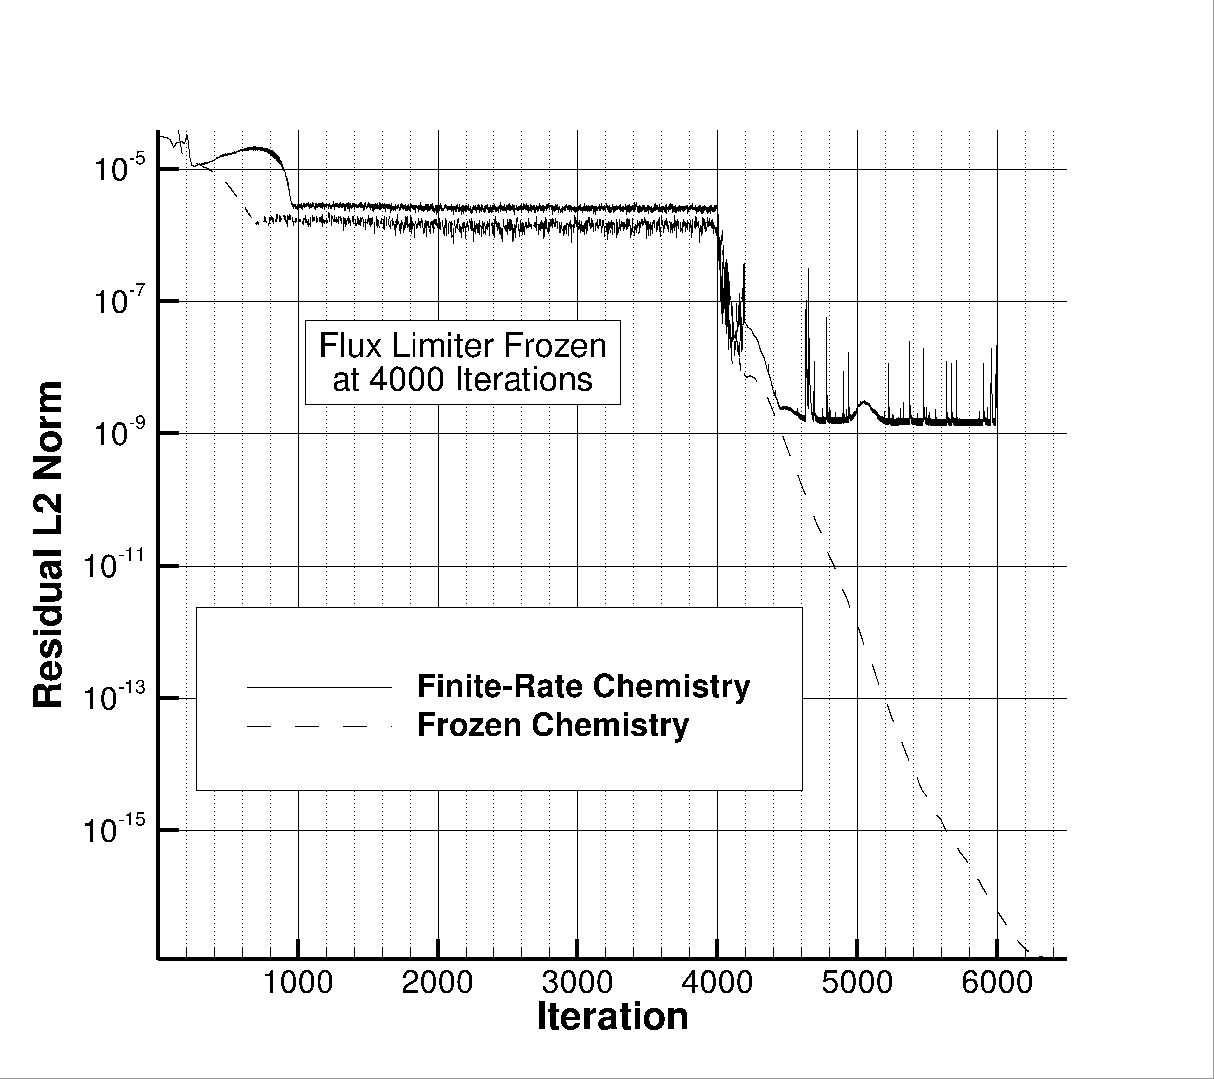
\includegraphics[width=0.5\textwidth]{figures/limiters/chem-res-comp.png}
  \caption{Typical residual convergence behavior.}
  \label{fig:chem-res-comp}
\end{figure}
%------------------------------------------------------------------------------%
\fref{fig:chem-res-comp} shows a typical convergence history, obtained on a
coarse mesh, for the annular jet case with a flux limiter engaged.  If no
chemical reactions are allowed to take place, i.e. ``frozen'' flow, the residual
of all equations can be decreased to less than $10^{-16}$.  If finite rate
chemistry is included, convergence ends at $\sim 10^{-8}$.  The difference is
believed to be associated with the high degree of stiffness in the chemical
source terms.  The large reaction rates significantly increase the condition
number of the Jacobian, and further updates to the solution do not improve
convergence.  This is not a problem for the adjoint solution, as both levels of
convergence are sufficient to obtain a solution; however, the convergence of the
flow equations with chemistry is marred by the high degree of sensitivity to the
flux limiter used.  It can be seen in \fref{fig:chem-res-comp} that convergence
to steady state is less smooth when chemistry is involved, and this is directly
tied to the flux limiter field.  In FUN3D, the frozen flux limiter is
re-evaluated when a reconstruction is unrealisable.  This reevaluation causes
high-frequency errors, which manifest as ``spikes'' in the residual history.
Fortunately, the reevaluation is only needed at a small number of nodes (usually
$< 10$ nodes), so integrated aerothermodynamic quantities are unaffected by
these reevaluations when convergence to steady-state is reached.  It should be
noted that while the results presented here are only on the coarsest (baseline)
mesh level, the refined meshes also exhibit similar behavior.

Because the solution is not grid converged, there is a significant difference
between the first-order and second-order solutions; therefore, the choice flux
limiters presented in \sref{sec:2nd-order-reconstruction} has a large impact on
the solution.  
%------------------------------------------------------------------------------%
\begin{figure}[h]
  \centering
  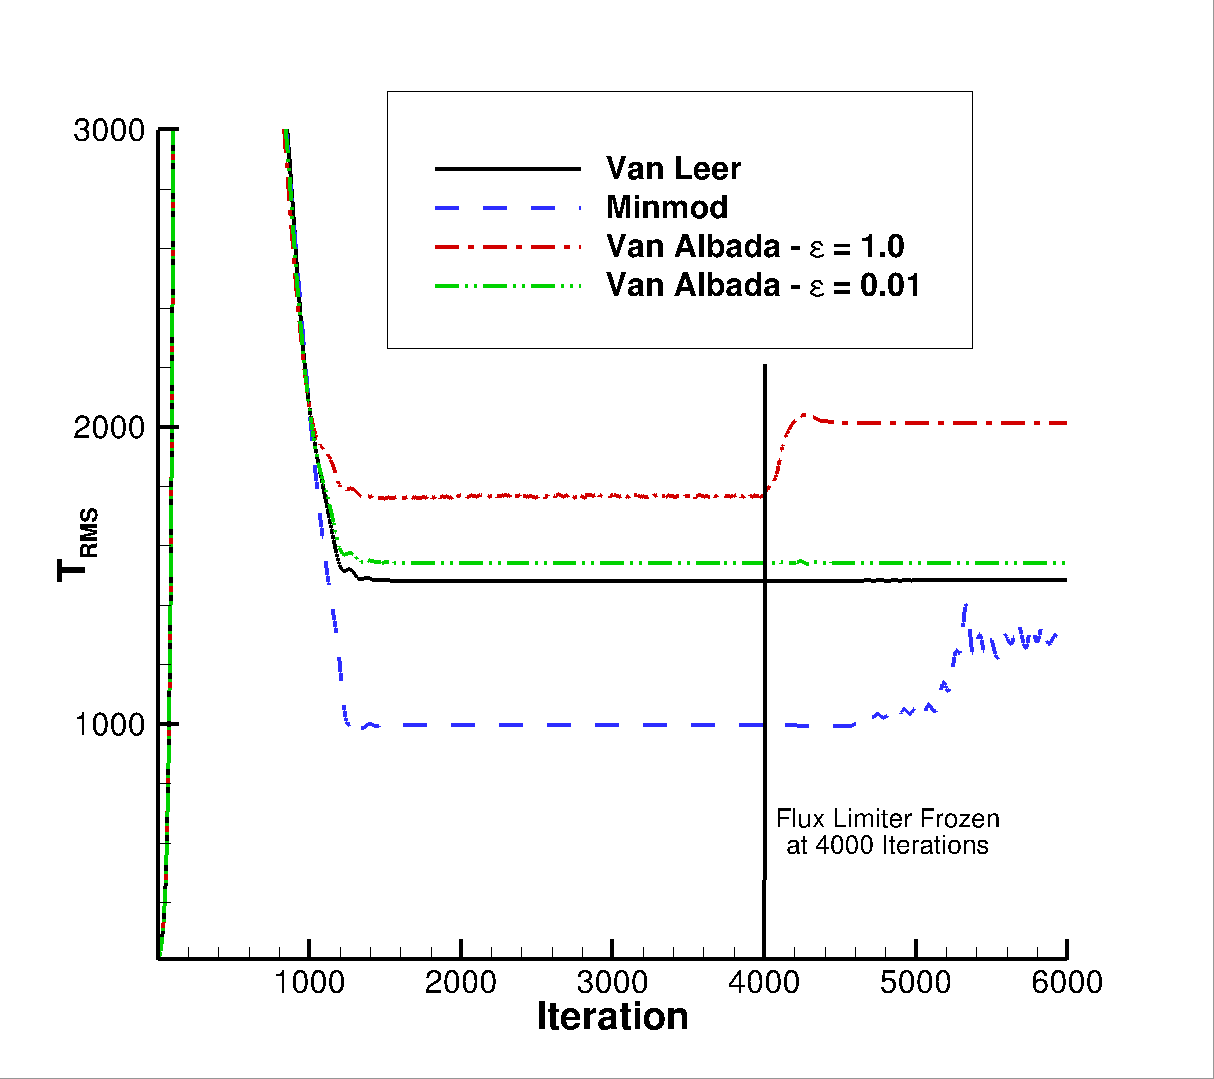
\includegraphics[width=0.5\textwidth]{figures/limiters/all-limiters.png}
  \caption{Convergence of surface temperature with different flux limiters.}
  \label{fig:all-limiters}
\end{figure}
%------------------------------------------------------------------------------%
\fref{fig:all-limiters} shows that the RMS of surface temperature on the outer
surface of the vehicle converges to significantly different results before
the flux limiter is frozen at iteration 4000.  The Minmod flux limiter exhibits
very large oscillations after freezing, due to the large number of non-smooth
reevaluations of the flux limiter where reconstructions became unrealisable.
These oscillations in the solution make the Minmod flux limiter unusable for
design optimization of this case. The Van Albada flux limiter converges to a
much more steady solution after being frozen; however, care must be taken to
``tune'' this particular limiter based the grid.  The tunable parameter,
$\varepsilon$, was evaluated at the recommended value of $1.0$, and was found to
increase the surface temperature by $> 20\%$ after freezing.  This is
unacceptable for design optimization, as it indicates a high dependence on
iteration that the flux limiter is frozen.
%------------------------------------------------------------------------------%
\begin{figure}[h]
  \centering
  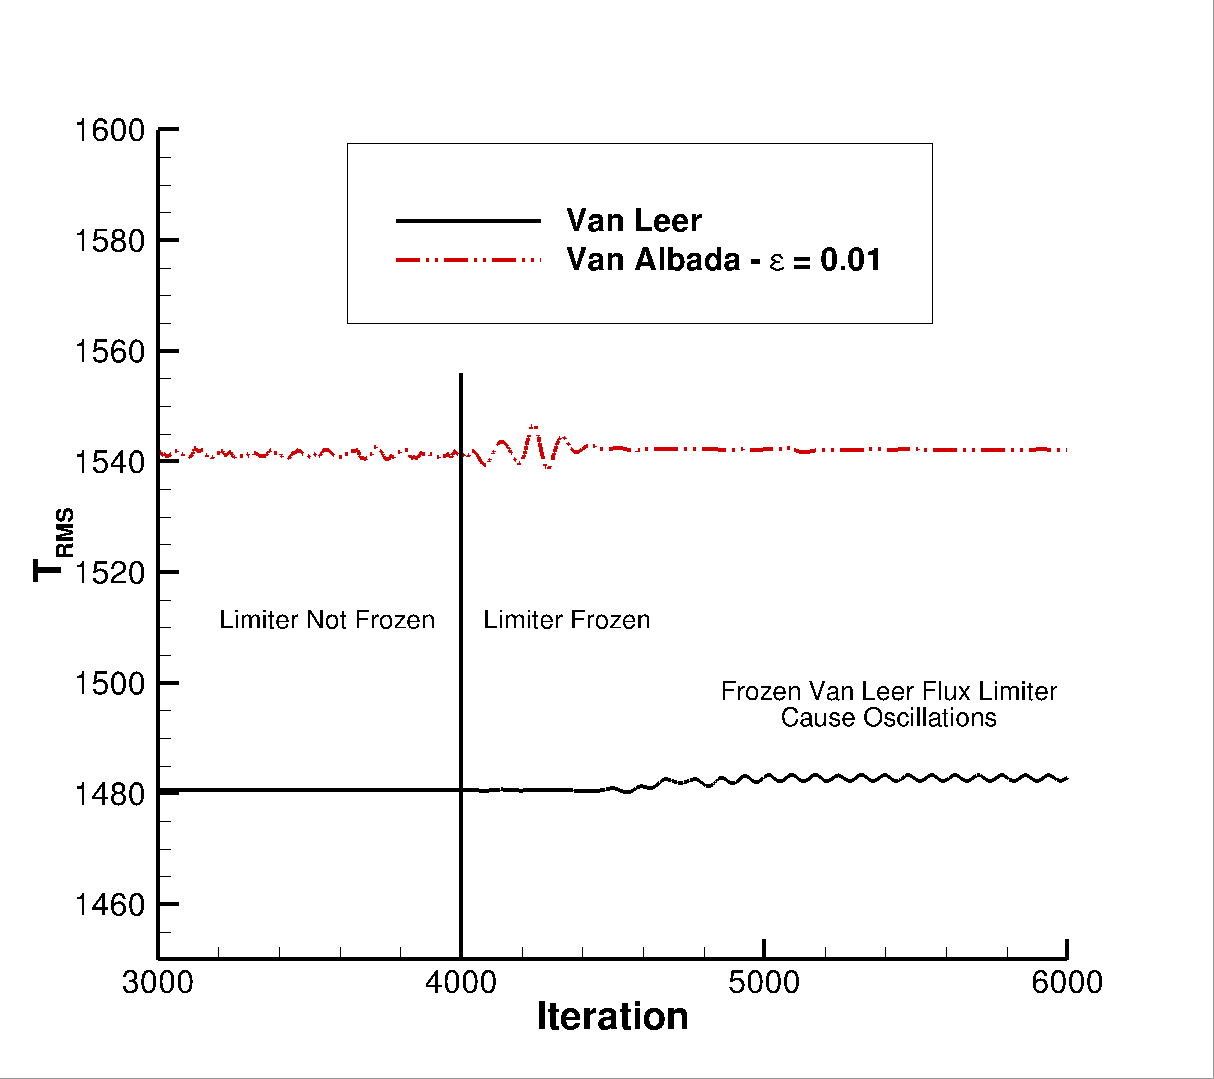
\includegraphics[width=0.5\textwidth]{figures/limiters/vanleer-vanalbada-frozen.png}
  \caption{Van Leer and Van Albada flux limiter impact on surface temperature.}
  \label{fig:vl-va-impact}
\end{figure}
%------------------------------------------------------------------------------%
The Van Leer flux limiter behaves much better in this regard; however,
\fref{fig:vl-va-impact} shows that the Van Leer limiter is also prone to
oscillations in the surface temperature RMS.  The oscillations are of small
enough amplitude that it might be reasonable to use the Van Leer flux limiter in
a design optimization of this problem, but a better alternative is to revisit
the Van Albada flux limiter.  \fref{fig:vl-va-impact} also shows that if
$\varepsilon$ is tuned to a value of $0.01$ the surface temperature RMS very
closely matches the average of the ringing value before the limiter was frozen.
For this reason, the Van Albada flux was used with $\varepsilon = 0.01$, which
tends towards the highly limited solution, as it seems to produce the most
steady result with the least dependence on the iteration that the flux limiter
is frozen.

None of the aforementioned flux limiter choices are ideal.  Because of the
sensitivity of the solution, attributable to freezing the limiter, the integrated
aerothermodynamic quantities demonstrated can vary between solutions with the
same inputs, but different starting states.  Tuning the Van Albada flux limiter
mitigates this issue, but does not solve it entirely, with some cases resulting
in a surface temperature RMS variance of $+/- 5 K$ with identical solver inputs
but different flow starting conditions. This is a recognized problem, but one
that is outside of the scope of this study.  A number of novel discretizations
at NASA Langley Research
Center\cite{gnoffo2014global,mazaheri2014very,mazaheri2016high} show promise in
mitigating or eliminating the need for a flux limiter, while achieving
higher-order spatial accuracy, and future work may incorporate them.
